\documentclass[12pt]{article}
\usepackage[margin=1in]{geometry} 
\usepackage{amsmath,amsthm,amssymb,amsfonts,algpseudocode,graphicx,mathtools}

\newcommand{\N}{\mathbb{N}}
\newcommand{\Z}{\mathbb{Z}}

\newenvironment{problem}[2][Problem]{\begin{trivlist}
\item[\hskip \labelsep {\bfseries #1}\hskip \labelsep {\bfseries #2.}]}{\end{trivlist}}
%If you want to title your bold things something different just make another thing exactly like this but replace ``problem'' with the name of the thing you want, like theorem or lemma or whatever

\newtheorem{theorem}{Theorem}
\newtheorem{lem}{Lemma}
\DeclarePairedDelimiter{\ceil}{\lceil}{\rceil}

\begin{document}
%\renewcommand{\qedsymbol}{\filledbox}
%Good resources for looking up how to do stuff:
%Binary operators: http://www.access2science.com/latex/Binary.html
%General help: http://en.wikibooks.org/wiki/LaTeX/Mathematics
%Or just google stuff

\title{CMPSCI-683 Homework Assignment \#4: Probabilistic Reasoning}
\author{Patrick Pegus II}
\maketitle

\textbf{Using an extension}

\begin{problem}{1}
	 It is quite often useful to consider the effect of some specific proposition in the context of
	 some general background evidence that remains fixed, rather than the complete absense of information.
	 \begin{enumerate}
		 \item Prove the conditionalized version of the general product rule: $P(X,Y|e) = P(X|Y,e)P(Y|e)$.\\
			 $P(X,Y|e)=\frac{P(X,Y,e)}{P(e)}=\frac{P(X,Y,e)}{P(Y,e)}\frac{P(Y,e)}{P(e)}=P(X|Y,e)P(Y|e)$
		 \item Prove the conditionalized version of Bayes' rule: $P(Y|X,e) = \frac{P(X|Y,e) P(Y|e)}{P(X|e)}$.\\
			 $P(Y|X,e)=\frac{P(Y,X,e)}{P(X,e)}=\frac{P(X|Y,e)P(Y,e)}{P(X|e)P(e)}=
			 \frac{P(X|Y,e)P(Y|e)P(e)}{P(X|e)P(e)}=\frac{P(X|Y,e) P(Y|e)}{P(X|e)}$
	 \end{enumerate}
\end{problem}
\begin{problem}{2}
	Suppose that you are given a bag containing $n$ unbiased coins.
	You are told that $n-1$ of these coins are normal, with heads on one side and tails on the other,
	whereas one coin is a fake, with heads on both sides.
	 \begin{enumerate}
		 \item Suppose you reach into the bag, pick out a coin at random, flip it, and get a head.
			 What is the (conditional) probability that the coin you chose is the fake coin?\\

			 Let $b$ be the event that the fake coin is chosen.
			 Let $f_1$ be the event that the first flip results in heads.
			 \begin{align*}
				 P(b|f_1)
				 &=\frac{P(f_1|b)P(b)}{P(f_1)}
				 =\frac{P(f_1|b)P(b)}{(n-1)P(f_1|\neg b)P(\neg b)+P(f_1|b)P(b)} \\
				 &=\frac{1 \cdot \frac{1}{n}}{(n-1)\frac{1}{2}\frac{n-1}{n}+1 \cdot \frac{1}{n}}
				 =\frac{2}{(n-1)^2+2}
			 \end{align*}
		 \item Suppose you continue flipping the coin for a total of $k$ times after picking it and see $k$ heads.
			 Now what is the conditional probability that you picked the fake coin?

			 \begin{align*}
				 P(b|f_k)
				 &=\frac{P(f_k|b)P(b)}{P(f_k)}
				 =\frac{P(f_k|b)P(b)}{(n-1)P(f_k|\neg b)P(\neg b)+P(f_k|b)P(b)} \\
				 &=\frac{1 \cdot \frac{1}{n}}{(n-1)\frac{1}{2^k}\frac{n-1}{n}+1 \cdot \frac{1}{n}}
				 =\frac{2^k}{(n-1)^2+2^k}
			 \end{align*}
		 \item Suppose you want to decide whether the chosen coin was fake by flipping it $k$ times.
			 The decision procedure returns fake if all $k$ flips come up heads; otherwise it returns normal.
			 What is the (unconditional) probability that this procedure makes an error?

			 \begin{align*}
				 P(e)=P(\neg b|f_k)=1-P(b|f_k)=1-\frac{2^k}{(n-1)^2+2^k}
			 \end{align*}
	 \end{enumerate}
\end{problem}
\begin{problem}{3}
	Consider the following Bayesian network:
	\begin{figure}[h]
		\centering
		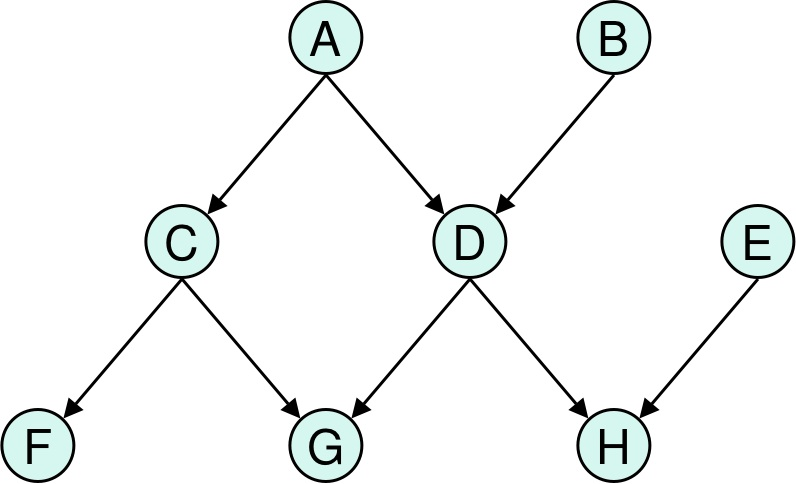
\includegraphics[width=0.5\textwidth]{fig/q3.jpg}
		%\caption{Nodes expanded and compute time as a function of the number of cities to be toured during 50 A$^*$ searches. The number of cities is a uniform random number between 1 and 15.}
		\label{fig:q3}
	\end{figure}
	 \begin{enumerate}
		 \item Suppose that all the variables are Boolean.
			 How many parameters (real numbers) are needed to specify an arbitrary joint probability distribution over 8 variables?
			 How many parameters are needed to define the joint probability distribution using the above Bayesian network?

			 $2^8-1$ parameters are needed to specify an arbitrary joint probability distribution.
			 With the given Bayesian network, 17 are needed (A-1, B-1, C-2, D-2, E-1, F-2, G-4, H-4).
		 \item
			 Which of the following probabilistic relations are implied by the structure of the above Bayesian network? Explain briefly.
			 \begin{enumerate}
				 \item $P(E|G) = P(E)$ Yes. Since $H$ is not evidence, $E$ is independent of all other nodes.
				 \item $P(C|D) = P(C)$ No. There is a flow of information along the path $D,A,C$.
				 \item $P(C|D,A) = P(C|A)$ Yes. Knowing $A$ and not knowing $G$ blocks all paths between $C$ and $D$.
				 \item $P(B|A,C) = P(B|A)$ Yes. Knowing $C$ and not knowing $D$ blocks all paths between $B$ and $A$.
				 \item $P(C,D|E) = P(C,D)$ Yes. Not knowing $H$ blocks all paths between $\{C,D\}$ and $E$.
				 \item $P(F|A,E,H) = P(F|A)$ Yes. Knowing $A$ and not knowing $G$ blocks all paths between $F$ and $\{E,H\}$.
				 \item $P(A,C|D,E,H) = P(A,C|D)$ Yes. Knowing $D$ and not knowing $G$ blocks all paths between $\{A,C\}$ and
					 $\{E,H\}$.
			 \end{enumerate}
		 \item  Express $P(A|G)$ in terms of the probabilities directly available in the network.
			 Simplify the expression as much as you can.
			 \begin{align*}
				 P(a|g)
				 &=\alpha P(a,g) \\
				 & =\alpha \sum_{b,c,d,e,f,h}P(a,g,b,c,d,e,f,h) \\
				 & =\alpha \sum_{b,c,d,e,f,h}P(a)P(g|c,d)P(b)P(c|a)P(d|a,b)P(e)P(f|c)P(h|d,e) \\
				 &=\alpha P(a)\sum_b P(b)\sum_e P(e)\sum_c P(c|A)\sum_d P(d|a,b)P(g|c,d)\sum_f P(f|c) \sum_h P(h|d,e) \\
				 &=\alpha P(a)\sum_b P(b)\sum_e P(e)\sum_c P(c|A)\sum_d P(d|a,b)P(g|c,d)
			 \end{align*}
	 \end{enumerate}
\end{problem}
\begin{problem}{4}
	Suppose that in a polytree network, $X$ is an ancestor of $Y$ and we wish to compute $P(Y|X)$
	in terms of the CPT entries of the network.
	Explain how this computation can be done as efficiently as possible and write a general expression for P(Y|X).
	(Hint: you may find it useful to consider an example such as the following,
	although the specific details of the example need not appear in your answer.) \\
	\begin{figure}[h]
		\centering
		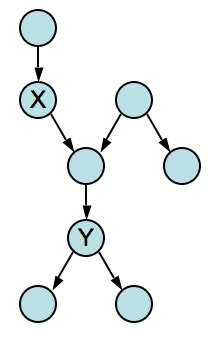
\includegraphics[width=0.125\textwidth]{fig/q4.jpg}
		%\caption{Nodes expanded and compute time as a function of the number of cities to be toured during 50 A$^*$ searches. The number of cities is a uniform random number between 1 and 15.}
		\label{fig:q4}
	\end{figure}

	Let $R=Parents(X)$.
	Let $A=Ancestors(Y) \cap Descendants(X)$.
	Let $P=Parents(A) \setminus A \setminus X$.
	Let $C=Children(A) \setminus A \setminus Y$.
	Let $D=Children(Y)$.
	$P(Y|X)$ is proportional to the marginal probability found when summing over $A$ and the
	Markov blanket surrounding $Y \cup X \cup A$, which is $R \cup P \cup C \cup D$ as in:
	\begin{align*}
		P(y|x)
		&=\alpha \sum_{r_i \in R}\sum_{a_i \in A}\sum_{p_i \in P}\sum_{c_i \in C}\sum_{d_i \in D}
		P(y,x,r_1,\dots,r_k,a_1,\dots,a_l,p_1,\dots,p_m,c_1,\dots,c_n,d_1,\dots,d_o)
	\end{align*}
\end{problem}
\begin{problem}{5}
	Suppose that in a Bayesian network containing an unobserved (non-evidence) variable $Y$,
	all the variables in the Markov blanket $MB(Y)$ have been observed.
	\begin{enumerate}
		\item Prove that removing the node Y from the network will not affect the posterior distribution
			for any other unobserved variable in the network.
			``This question is a bit open ended, and is not very specific about what “remove” means.
			When a node is a leaf node with no children, removing it and its CPT leaves the rest of the network unchanged.
			When a node has children, however, we have to decide what to do about the CPTs of those children,
			since one parent has disappeared.
			The only reasonable interpretation is that removal has to leave the posterior of all other variables unchanged
			regardless of what new CPTs are supplied for Y's children.''

			Let $A$ be the set of all nodes in the network.
			Let $O=A \setminus MB(Y) \setminus Y$.
			Let $C=Children(Y)$.
			Let $Z=MB(Y) \setminus C$.
			Let $Par(N)$ be the parents of node $N$.
			\begin{align*}
				P(x|MB(Y))
				&=\alpha\sum_{o_i \in O}\sum_y P(x,o_1,\dots,o_l,z_1,\dots,z_m,c_1,\dots,c_n,y) \\
				%&=\alpha\sum_{o_i \in O}\sum_y P(x,o_1,\dots,o_l,z_1,\dots,z_m,c_1,\dots,c_n|y)P(y) \\
				%&=\alpha\sum_{o_i \in O}P(x,o_1,\dots,o_l,z_1,\dots,z_m,c_1,\dots,c_n \\
				&=\alpha\sum_{o_i \in O}\sum_y P(x,o_1,\dots,o_l,z_1,\dots,z_m|c_1,\dots,c_n,y)P(c_1,\dots,c_n,y) \\
				&=\alpha\sum_{o_i \in O}\sum_y P(x,o_1,\dots,o_l,z_1,\dots,z_m|c_1,\dots,c_n)P(c_1,\dots,c_n,y) \text{, by d-separation}\\
				&=\alpha\sum_{o_i \in O} P(x,o_1,\dots,o_l,z_1,\dots,z_m|c_1,\dots,c_n)\sum_y \prod_{i=1}^n P(c_i|Par(c_i))P(y|Par(Y)) \\
				&=\alpha\sum_{o_i \in O} P(x,o_1,\dots,o_l,z_1,\dots,z_m|c_1,\dots,c_n)\sum_y \prod_{i=1}^n P(c_i|Par(c_i)\setminus Y,Y)P(y|Par(Y)) \\
				&=\alpha\sum_{o_i \in O} P(x,o_1,\dots,o_l,z_1,\dots,z_m|c_1,\dots,c_n)\sum_y \prod_{i=1}^n P(c_i|Par(c_i)\setminus Y,Y)P(y|Par(Y)) \\
				&=\alpha\sum_{o_i \in O} P(x,o_1,\dots,o_l,z_1,\dots,z_m|c_1,\dots,c_n) \prod_{i=1}^n P(c_i|Par(c_i)\setminus Y) \\
				%&=\alpha\sum_{o_i \in O} P(x,o_1,\dots,o_l,z_1,\dots,z_m|c_1,\dots,c_n)\sum_y \prod_{i=1}^n P(c_i|Parents(c_i))P(y) \\
				%&=\alpha\sum_{o_i \in O} P(x,o_1,\dots,o_l,z_1,\dots,z_m|c_1,\dots,c_n)\sum_y P(c_1,\dots,c_n|y)P(y) \\
				%&=\alpha\sum_{o_i \in O} P(x,o_1,\dots,o_l,z_1,\dots,z_m|c_1,\dots,c_n)P(c_1,\dots,c_n) \\
			\end{align*}
		\item Discuss whether we can remove Y if we are planning to use (i) rejection sampling and (ii) likelihood weighting.

			%As long as the conditional probability tables of $Y$'s children were updated so that $Y$ is not included, we
			%could sample all nodes in $MB(Y)$ and reject those that do not agree with the evidence, for successful rejection sampling.
			%Similarly, we could weight the given values
			Since rejection sampling requires that we know the conditional probability of the children of $Y$ given their parents
			in order to generate a sample, which would then be accepted if it matched the evidence, $Y$ cannot be removed.
			Similarly in likelihood weighting, we use those conditional probabilities to generate the weight for the given
			evidence, which again requires that we know the value of $Y$.
	\end{enumerate}
\end{problem}
\begin{problem}{6}
	You are an AI consultant for an auto insurance company. Your task is to construct a Bayesian network that will allow the company to decide how much financial risk they run from various policy holders, given certain data about the policy holders. In order to design a Bayesian network, you need output variables and evidence variables. The output variables are those for which the insurance company is trying to get a probability distribution for their possible values. The evidence variables are those variables for which you can obtain information, on the basis of which it is legal to make decisions, and that are relevant to the decision. Output variables represent the cost of various catastrophic events that the insurance company might have to reimburse. In the automobile insurance domain, the major output variables are the medical cost (MedCost), property cost (PropCost), and intangible liability cost (ILiCost). Medical and property costs are those incurred by all individuals involved in an accident; auto theft or vandalism might also incur property cost. Intangible liability costs are legal penalties for things like``pain and suffering,'' punitive damages, and so forth, that a driver might incur in an accident in which he or she is at fault. Evidence variables for this domain include the driver's age and record; whether or not he or she owns another car; how far he or she drives per year; the vehicle's make, model and year; whether it has safety equipment such as airbag and antilock brakes; where it is garaged and whether it has an antitheft device.
	\begin{enumerate}
		\item Build a possible belief network for this problem. You will need to decide on suitable domains for the variables, bearing in mind the need to discretize. You will also need to add intermediate nodes such as DrivingSkill and AutoRuggedness.
			\begin{figure}[h]
				\centering
				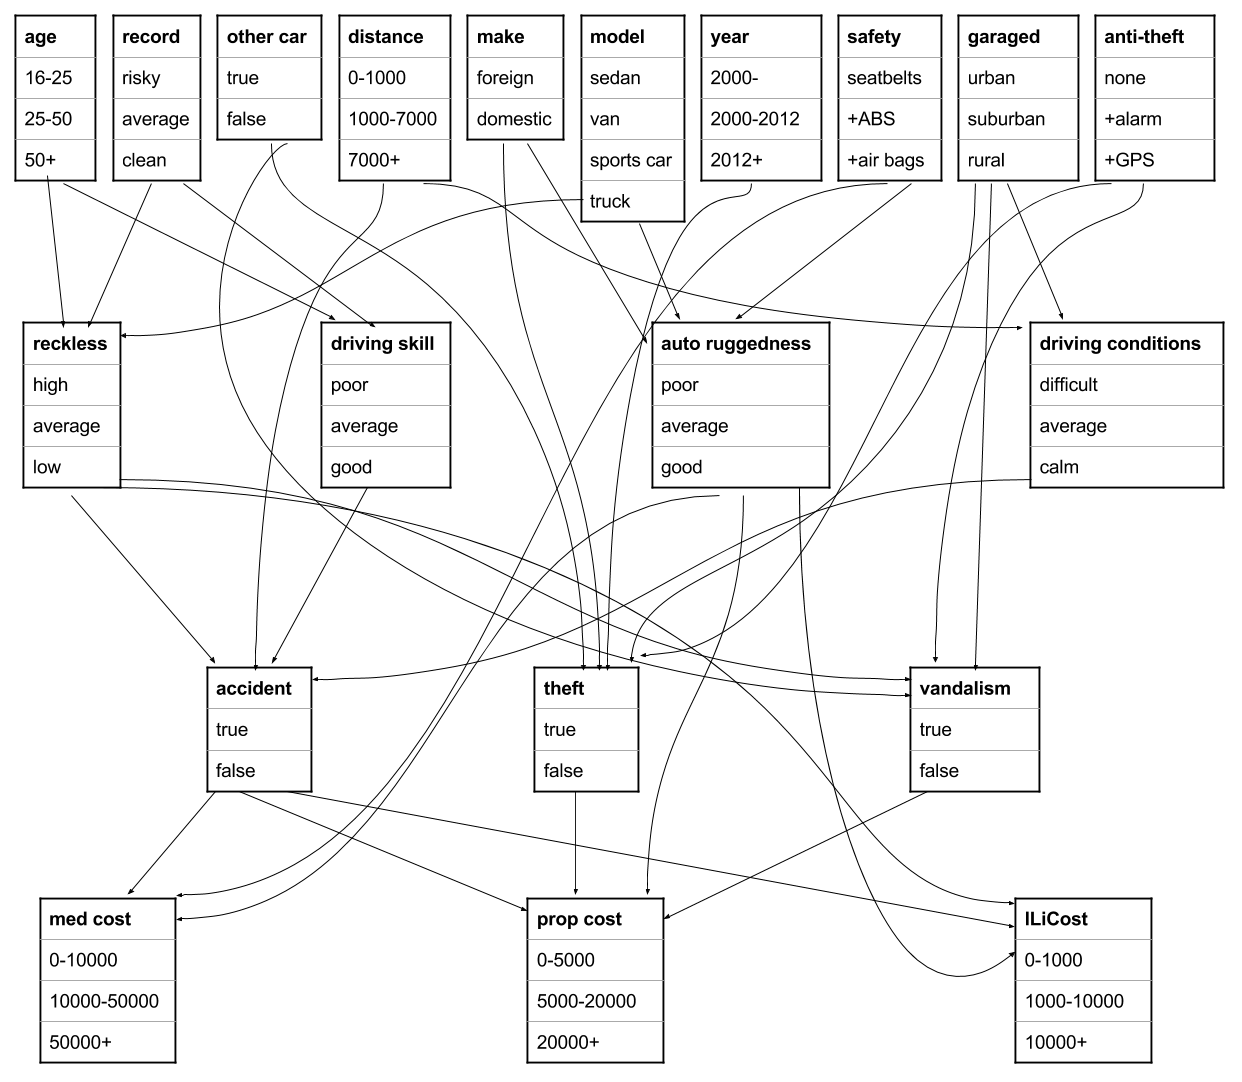
\includegraphics[width=0.875\textwidth]{fig/hw4-6.png}
				%\caption{Nodes expanded and compute time as a function of the number of cities to be toured during 50 A$^*$ searches. The number of cities is a uniform random number between 1 and 15.}
				\label{fig:q6}
			\end{figure}
		\item Give reasonable conditional probability tables to a few (but not all!) nodes.

			The following is a CPT for driving skill.\\
			\begin{tabular}{|c|c|c|c|c|}
				\hline
				high & average & age & record \\
				\hline
				.95 & .04 & 16-25 & risky \\
				.7 & .2 & 25-50 & risky \\
				.75 & .22 & 50+ & risky \\
				.9 & .06 & 16-25 & average \\
				.6 & .3 & 25-50 & average \\
				.55 & .4 & 50+ & average \\
				.5 & .4 & 16-25 & clean \\
				.1 & .2 & 25-50 & clean \\
				.01 & .1 & 50+ & clean \\
				\hline
			\end{tabular}
		\item How many independent values are necessary to define the joint probability distribution of your model, assuming no conditional independence relations hold among the variables? How many independent values are needed to complete your model using the conditional independence relations?

			If no conditional independence relations hold, the full joint distribution must be specified,
			which requires 612220031 values.
			Using the conditional independence relations of the model, 346 values are required.
	\end{enumerate}
\end{problem}
\begin{problem}{7}
\end{problem}

\end{document}
